\chapter[Least squares]{More on the method of least squares}
The method of least squares is one the most important and pervasive topics in applied linear algebra. Dues to it's relevance and importance the topic demands a second look.

To begin, the name of the method stems from two facts:
\begin{enumerate}
\item \textit{least} implies minimization, which implies distance, which implies norm,
\item {squares} implies the $L_{2}$ norm, the quadratic summation of Pythagoras.
\end{enumerate}

\section{Methods}

Consider the case of overdetermined systems; these are cases where we have more data points than parameters. The linear system is this
\begin{equation*}
  \ls
\end{equation*}
where $\Amnrr$, the fit parameters $x\in\cmplxm$



\endinput
\section{The general solution}

Let's resume the discussion with the issue posed in \S\eqref{sec:pi}. The issue was the general system to the linear system given by 
$$
\ls.
$$
By generalizing the matrix inverse we were able to solve the general problem. THe target matrix did not have to be square; it was no longer restricted to being nonsingular. This general solution was expressed in equation \eqref{eq:solution:general}:
$$
    \Ap\paren{\A{}x} = \A{+}b.
$$
We were troubled by the fact that the matrix product on the left-hand side is in general not an identity matrix:
\begin{equation}
  \Ap\A{} \ne \I{n}.
\end{equation}
(Later on in \S\eqref{sec:chiral} we saw that the pseudoinverse is a left inverse
\begin{equation}
  \Ap\A{} = \I{n}
\end{equation}
when the target matrix has full column rank.) We also went on to discover in \S\eqref{sec:solution:complete} that while $\A{+}b$ is the point solution, it is not the complete solution as seen, for example, in equation \eqref{eq:simple:fullsoln}.

Now armed with the knowledge of the four fundamental projectors from \S\eqref{sec:orthproj} we can bring this issue into full theoretical appreciation. In equation \eqref{eq:fourprojpi} we saw that the matrix product of interest is the operator which projects vectors onto the perpendicular complement of the of the null space of the target matrix:
\begin{equation}
  \projnap = \leftinv.
\end{equation}


\endinput
\section{Solution using the SVD}
Let's return to using an SVD to solve the linear systems like $\ls$ as shown in \S\eqref{sec:formal:simple}.

Once you have the SVD life is good.
 
%%
\subsection{Extended example SVD}
We don't want 3 x 3, go to 3 x 5
\begin{equation}
  \begin{array}{cccc}
    \A{}&x &=& b\\
    \mat{rrrrr}
    {
     1 & -1 &  1 & -1 &  1\\
    -1 &  1 & -1 &  1 & -1\\
     1 & -1 &  1 & -1 &  1\\
    }
    &
    \mat{c}{x_{1}\\x_{2}\\x_{3}\\x_{4}\\x_{5}}
    &=& \phivector.
  \end{array}
\end{equation}

\textbf{Recycling:} The good news is that we can solve this system using the simple \svdl \ method of the first chapter allowing us to bypass the eigensystem problem. Even more good] news is that we can recycle the codomain matrix $\Y{}$. The active column vector in the domain matrix is this:
\begin{equation}
  \X{}_{*,1} = \sfive\mat{r}{1 \\ -1 \\  1 \\ -1 \\  1}.
\end{equation}
Using the fact that
\begin{equation}
  \begin{split}
    \A{}\X{}_{*,1}=\sigma_{1}\Y{}_{*,1}
  \end{split}
\end{equation}
we can compute the lone singular value of
\begin{equation}
  \sigma_{1} = 15^{-1/2}.
\end{equation}

Without doing noticeable calculation, we already have the partial decomposition
\begin{equation}
  \begin{split}
    \svda{T}\\
    &=
    \Yshade
    \mat{c|cccc}
    {
     15^{-1/2} & 0 & 0 & 0 & 0\\\hline
      0 & 0 & 0 & 0 & 0\\
      0 & 0 & 0 & 0 & 0\\
    }
    \mat{ccccc}
    {\sfive & -\sfive & \phantom{-}\sfive & -\sfive & \phantom{-}\sfive\\
     \rowcolor{ltgray}
     \cdot  &  \phantom{-}\cdot  & \phantom{-}\cdot  &  \phantom{-}\cdot  & \phantom{-}\cdot \\
     \rowcolor{ltgray}
     \cdot  &  \phantom{-}\cdot  & \phantom{-}\cdot  &  \phantom{-}\cdot  & \phantom{-}\cdot \\
     \rowcolor{ltgray}
     \cdot  &  \phantom{-}\cdot  & \phantom{-}\cdot  &  \phantom{-}\cdot  & \phantom{-}\cdot \\
     \rowcolor{ltgray}
     \cdot  &  \phantom{-}\cdot  & \phantom{-}\cdot  &  \phantom{-}\cdot  & \phantom{-}\cdot}\\
  \end{split}
\end{equation}

The Gram-Schmidt process in the appendix \eqref{sec:gs} will complete the $\X{}$ matrix. Using the seed vectors
\begin{equation}
  U = \lst{
  \mat{r}{1 \\ -1 \\  1 \\ -1 \\  1},
  \mat{c}{1\\0\\0\\0\\0},
  \mat{c}{0\\1\\0\\0\\0},
  \mat{c}{0\\0\\1\\0\\0},
  \mat{c}{0\\0\\0\\1\\0}
  }
\end{equation}
the domain matrix becomes
\begin{equation}
  \X{} = 
  \left[
\begin{array}{ r >{\columncolor{ltgray}}r >{\columncolor{ltgray}}r >{\columncolor{ltgray}}r >{\columncolor{ltgray}}c }
  \sfive &  \frac{4}{2\sqrt{5}} &  0 &  0 &  0 \\
 -\sfive &  \frac{1}{2\sqrt{5}} &  \frac{3}{2\sqrt{3}} &  0 &  0\\
  \sfive & -\frac{1}{2\sqrt{5}} &  \frac{1}{2\sqrt{3}} & -\frac{2}{6} &  0\\
 -\sfive &  \frac{1}{2\sqrt{5}} & -\frac{1}{2\sqrt{3}} &  \ssix & \stwo\\
  \sfive & -\frac{1}{2\sqrt{5}} &  \frac{1}{2\sqrt{3}} & -\ssix & \stwo\\
\end{array}
\right]
\end{equation}

Now do the change of coordinates stuff in the section on a more formal introduction.
 
%%
\subsection{Extended example solution}
The particular solution for the problem is given by this
\begin{equation}
  x_{p} = \A{+}b.
  \label{eq:lsq:a}
\end{equation}
Since the domain matrices are mainly composed of null vectors, the pseudoinverse is a quick construction. We need only one outer product
\begin{equation}
  \begin{split}
    \A{+} &= \sigma_{1}\X{}_{*,1}\otimes \Y{T}_{1,*}\\
     &= \paren{15^{-1/2}}
     \paren{\sfive \mat{r}{1\\-1\\1\\-1\\1}}
     \paren{\sthree \mat{rrr}{1&-1&1}} =
     \frac{1}{15}\mat{rrr}{1 & -1 & 1\\-1 & 1 & -1\\1 & -1 & 1\\-1 & 1 & -1\\1 & -1 & 1}.
  \end{split}
\end{equation}
The point solution, the particular solution, of equation \eqref{eq:lsq:a} is then
\begin{equation}
  x_{p} = \frac{1}{15}\mat{rrrrr}{1 & -1 & 1 & -1 & 1}^{\mathrm{T}}.
\end{equation}
The homogenous solutions add considerable flavor to the full solution. The null space is spanned by four vectors.
\begin{equation}
  \begin{split}
    x &= x_{p} + x_{h}\\
      &= \underbrace{\frac{1}{15}\mat{r}{1\\-1\\1\\-1\\1}}_{\text{particular}}
       + \underbrace{
         \alpha_{1}  \mat{r}{4\\1\\-1\\1\\-1} 
       + \alpha_{2}  \mat{r}{0\\3\\1\\-1\\1} 
       + \alpha_{3}  \mat{r}{0\\0\\-2\\1\\-1} 
       + \alpha_{4}  \mat{r}{0\\0\\0\\1\\1}
         }_{\text{homogeneous}} 
  \end{split}
\end{equation}
where the constants $\alpha$ are arbitrary complex numbers.
 
%%
\subsection{Extended example solution}
Using the coordinate transformations of equation \eqref{eq:moreformal:a}
\begin{equation*}
  \begin{split}
    \mathbb{X} & = \X{*} x  \\
    \mathbb{B} & = \Y{*} b
    \label{eq:moreformal:a}
  \end{split}
\end{equation*}
The $\mathbb{B}$ vector is unchanged from equation \eqref{eq:morefomal:B}
\begin{equation*}
    \mathbb{B} = \mat{r}{\sthree \\ \stwo \\ \frac{-2}{\sqrt{6}}}.
\end{equation*}
The new $\mathbb{X}$ vector is now given by this
\begin{equation}
  \mathbb{X} = \mat{c}{
  \frac{1}{\sqrt{5}}\paren{x_{1}+2x_{2}} \\
 -\frac{1}{\sqrt{5}}x_{1}+\frac{1}{2\sqrt{5}}x_{2}+\frac{\sqrt{3}}{2}x_{3} \\
  \frac{1}{\sqrt{5}}x_{1}-\frac{1}{2 \sqrt{5}}x_{2}+\frac{1}{2 \sqrt{3}}x_{3}+\sqrt{\frac{2}{3}} x_{4}\\[5pt]
 -\frac{1}{\sqrt{5}}x_{1}+\frac{1}{2 \sqrt{5}}x_{2}-\frac{1}{2 \sqrt{3}}x_{3}+\frac{1}{\sqrt{6}}x_{4}+\frac{1}{\sqrt{2}}x_{5}\\[5pt]
  \frac{1}{\sqrt{5}}x_{1}-\frac{1}{2 \sqrt{5}}x_{2}+\frac{1}{2 \sqrt{3}}x_{3}-\frac{1}{\sqrt{6}}x_{4}+\frac{1}{\sqrt{2}}x_{5}
  }.
\end{equation}

The simplified solution of equation \eqref{eq:formal:svdsoln} is given by
\begin{equation}
  \begin{split}
    \mathbb{X} &= \sig{(+)}\, \mathbb{B}\\
    \mat{r}{
    \sfive            \paren{x_{1} - x_{2} + x_{3} - x_{4} + x_{5}} \\
    \frac{2}{\sqrt{5}}\paren{4x_{1}+ x_{2} - x_{3} + x_{4} - x_{5}} \\
    \frac{2}{\sqrt{3}}\paren{       3x_{2} + x_{3} - x_{4} + x_{5}} \\
    \ssix             \paren{              -2x_{3} + x_{4} - x_{5}} \\
    \stwo             \paren{                        x_{4} + x_{5}} \\
  }
  &= \mat{c}{\sqrt{5}\\[5pt]0\\[5pt]0\\[5pt]0\\[5pt]0}
  \end{split}
\end{equation}

\endinput
\section{A curious example}

We have seen the power of the method of least squares: for systems without direct solutions we can always find least squares solutions. The embodiment of this capability is the pseudoinverse which orthogonally projects the data vector down onto the range thereby finding the solution in the range closest to the data. Here we present a curious example as a probe of the pseudoinverse in the method of least squares. Suppose the data. We are begging the question: where do two parallel lines meet in the plane $\real{2}$?

%%
\subsection{The problem}
Consider two functions
\begin{equation}
\begin{split}
  f_{1}(x) &= -x,\\
  f_{2}(x) &= -x + 1,
\end{split}
\end{equation}
which define two parallel lines with unit offset. We know the lines do not cross, yet we also know the method of least squares will create a solution point. Where is this solution point?

%%
\subsection{The problem}
The linear system is given by this
\begin{equation}
  \begin{split}
    \lsa\\
    \mat{cc}{1&1\\1&1}\mat{c}{x\\y} &= \mat{c}{0\\1}.
  \end{split}
\end{equation}There is one independent row vector $r_{1}$:
\begin{equation}
  \mat{cc}{1&1\\\hline1&1} = \mat{c}{r_{1}^{\mathrm{T}}\\\hline r_{1}^{\mathrm{T}}}, \qquad r_{1}=\mat{c}{1\\1}.
\end{equation}
The orthogonal complement vectors are given by this
\begin{equation}
  r_{1}^{\perp} = \alpha\mat{r}{-1\\1}, \quad \alpha \in \cmplx{}.
\end{equation}
Without any loss of generality, set
\begin{equation}
  \alpha = 1.
\end{equation}
The candidate domain matrix then
\begin{equation}
  \X{} = 
\stwo
\left[
\begin{array}{r >{\columncolor{ltgray}}r}
  1 & -1 \\
  1 &  1
\end{array}
\right]
.
\end{equation}

In a similar fashion there is one independent column vector $c_{1}$:
\begin{equation}
  \mat{c|c}{1&1\\1&1} = \mat{c|c}{c_{1}&c_{1}}, \qquad c_{1}=\mat{c}{1\\1}.
\end{equation}
While this has the same value as the vector $r_{1}$, remember that the row vector $r_{1}$ is in the domain (solution space) and the column vector is in the codomain $c_{1}$ (measurement space).

Location aside, the same image vector allows us to use the same perpendicular complement. The result is the codomain matrix
\begin{equation}
  \Y{} = 
\stwo
\left[
\begin{array}{r >{\columncolor{ltgray}}r}
  1 & -1 \\
  1 &  1
\end{array}
\right]
.
\end{equation}

The lone eigenvalue comes from this relationship:
\begin{equation}
  \begin{split}
    \A{} \X{}_{*,1} &= \sigma_{1} \Y{}_{*,1},\\
    \frac{2}{\sqrt{2}}
    \mat{c}{1\\1} &= \frac{\sigma_{1}}{\sqrt{2}}
    \mat{c}{1\\1}.
  \end{split}
\end{equation}

Therefore $\sigma_{1} = 2$ and we can write the SVD for the target matrix:
\begin{equation}
  \begin{split}
     \svda{T}\\
     \mat{cc}{1&1\\1&1} &= 
     \stwo
\left[
\begin{array}{r >{\columncolor{ltgray}}r}
  1 & -1 \\
  1 &  1
\end{array}
\right]
     \mat{c|c}{2&0\\\hline 0&0}
     \stwo \mat{rr}{1&1\\\rowcolor{ltgray}-1&1}.
  \end{split}
\end{equation}

The point of the decomposition was to assemble the pseudoinverse:
\begin{equation}
  \begin{split}
     \mpgia{T}\\
      \rtwo \mat{cc}{1&1\\1&1} &= 
\stwo
\left[
\begin{array}{r >{\columncolor{ltgray}}r}
  1 & -1 \\
  1 &  1
\end{array}
\right]
     \mat{c|c}{\frac{1}{2}&0\\[3pt]\hline 0&0}
     \stwo \mat{rr}{1&1\\\rowcolor{ltgray}-1&1}.
  \end{split}
\end{equation}

The general solution to the least squares problem is written as the following:
\begin{equation}
\boxed{
  \begin{array}{rccccc}
    x_{gen} &=& x_{p} &\oplus& x_{h},\\[7pt]
      &=& \A{+}b &\oplus& \alpha \X{}_{*,2}, & \alpha\in\cmplx{}\\[7pt]
      &=& \frac{1}{4}\mat{r}{1\\1} &\oplus& \alpha \mat{r}{-1\\1}\\[17pt]
      &=& \textit{point} &\oplus& \textit{line}
  \end{array}
}
\label{eq:simple:fullsoln}
\end{equation}

\clearpage
\begin{table}[htdp]
\begin{center}
\begin{tabular}{ccc}
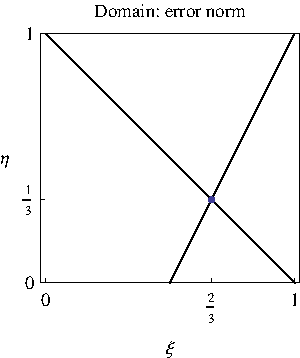
\includegraphics[ width = 1.5in ]{pdf/lsq/direct_fcns} &
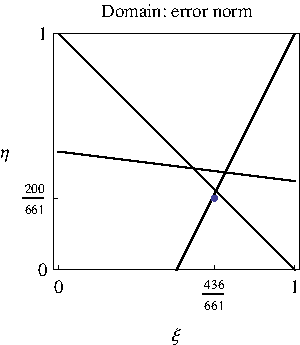
\includegraphics[ width = 1.5in ]{pdf/lsq/three_fcns}  &
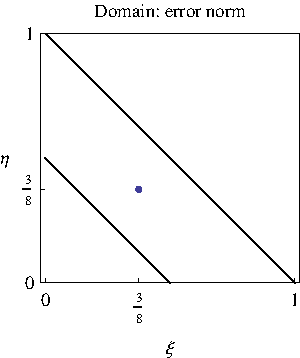
\includegraphics[ width = 1.5in ]{pdf/lsq/parallel_fcns}\\
$y_{1}(x) = -x+1$ & $y_{1}(x) = -x+1$ & $y_{1}(x) = -x+1$\\
$y_{2}(x) = 2x-1$ & $y_{2}(x) = 2x-1$ & $y_{4}(x) = -x+\frac{1}{2}$\\
 & $y_{3}(x) = -\frac{1}{8}x+\frac{3}{2}$ \\
\textellipsis & \textellipsis & \textellipsis \\
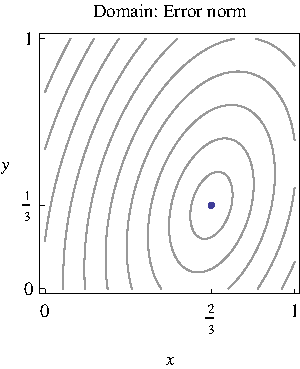
\includegraphics[ width = 1.5in ]{pdf/lsq/direct_error} &
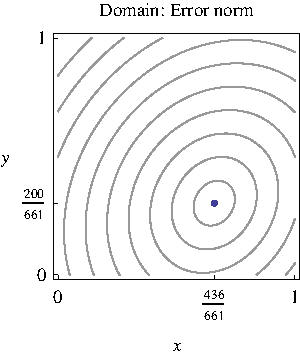
\includegraphics[ width = 1.5in ]{pdf/lsq/three_error}  &
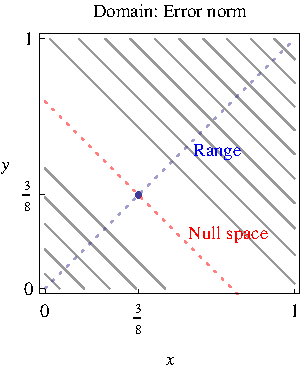
\includegraphics[ width = 1.5in ]{pdf/lsq/parallel_error}\\
\textellipsis & \textellipsis & \textellipsis \\
$\A{} = \mat{rr}{1&1\\-2&1}$ &
$\A{} = \mat{rr}{1&1\\-2&1\\1/8&3/8}$ &
$\A{} = \mat{cc}{1&1\\1&1}$ \\
$\Ap = \AinvB = $ &
$\Ap = \AinvL = $ &
$\Ap = $ \\
$\rthree\mat{rr}{2&-1\\1&1}$ &
$\frac{1}{1322}\mat{rrr}{324&-492&122\\373&217&498}$ &
$\frac{1}{4}\mat{cc}{1&1\\1&1}$ \\
\textellipsis & \textellipsis & \textellipsis \\
\textellipsis & \textellipsis & \textellipsis \\
\end{tabular}
\end{center}
\caption{default}
\label{tab:curious:all}
\end{table}%

\clearpage


%%
\subsection{Interpretation}


\endinput
\section{0, 1, $\infty$}
Consider the generic linear system
\begin{equation*}
  \ls
\end{equation*}
where
\begin{equation}
  \Accmn, \quad x\in\cmplx{n}, \quad b\in\cmplx{m}.
\end{equation}

Let us consider these systems without recourse to least squares of the SVD.
A foundation tenet of linear algebra classifies linear systems as having three possible solutions:
\begin{enumerate}
\item No solution: there is no vector $x$ which satisfies the linear system.
\item A unique solution: there is a unique vector $x$ which satisfies the linear system.
\item An infinitude of solutions: there is an infinite number of vectors $x$ which satisfies the linear system.
\end{enumerate}

%%%
\subsection{A unique solution}
There are three general cases where we expect a unique solution. We start with the obvious case where the system matrix $\A{}$ is nonsingular. Then we explore two cases where there is some form of rank deficiency.

%%%
\subsubsection{Nonsingular system matrix}
All nonsingular matrices offer a direct solution of the form
\begin{equation}
  x = \A{-1}b
\end{equation}
where the vector $x$ is unique. These are the first cases we studied in linear algebra. How can we see that the solution is unique? One way is to employ proof by contradiction. Assume that there are two solutions, $x_{1}$ and $x_{2}$. By proposition
\begin{equation}
  \begin{split}
    \A{}x_{1} & = b \quad \Rightarrow \quad x_{1} = \A{-1}b, \\
    \A{}x_{2} & = b \quad \Rightarrow \quad x_{2} = \A{-1}b.
  \end{split}
\end{equation}
Subtract the two equations to find
\begin{equation}
  \A{}\paren{x_{1} - x_{2}} = \zero \qquad  \Rightarrow\Leftarrow,
\end{equation}
The contradiction comes because the last equation implies that.

%%%
\subsubsection{System matrix with full column rank}
The domain space $\cmplx{n\times n}$ is spanned by two $\nv$s. The null space for the domain is trivial.
This implies that there are no null vectors in the domain matrix $\X{}$:
\begin{equation}
  \A{} = \mat{rr}{1&1\\-1&1\\1&1}
\end{equation}
\begin{equation}
  \begin{split}
    \svda{T} \\
    \mat{rr}{1&1\\-1&1\\1&1} & = 
\mat{cc>{\columncolor{ltgray}}c}{\stwo & 0 & \nstwo \\ 0 & 1 & 0 \\ \stwo & 0 & \nstwo}
\mat{cc}{2 & 0 \\ 0 & \sqrt{2} \\\hline 0 & 0 }
\mat{cc}{\stwo & \stwo \\ \nstwo & \stwo}
  \end{split}
\end{equation}

The least squares solution is then
\begin{equation}
\begin{split}
  \Ap b & = x,\\
  \rtwo \mat{crc}{1 & -2 & 1 \\ 1 & 2 & 1} \phivector &= \mat{c}{0\\1}
\end{split}
\end{equation}
There is no null space for the matrix $\A{}$. Hence there are no sull space vectors to add to the solution: the solution is unique. 

Notice the action when the pseudoinverse is the left inverse as in this case:
\begin{equation}
  \begin{split}
    \A{}x & = b, \\
    \Ap\A{}x & = \Ap b, \\
    \I{n} x & = \Ap b, \\
    \therefore x & = \Ap b, \\
  \end{split}
\end{equation}


%%%
\subsubsection{Rank deficient system matrix}
Consider the following linear system. The target matrix $\A{}$ has one unique column, therefore the matrix rank $\rho = 2$ and the matrix inverse $\A{-1}$ does not exist.
\begin{equation}
  \mat{cc}{\alpha & \alpha \\ \beta & \beta} \mat{c}{x_{1}\\x_{2}} = \mat{c}{b_{1}\\b_{2}}
\end{equation}
where $\alpha$ and $\beta$ are arbitrary complex numbers.
However, if the data vector lines on the range of the target matrix $\rng{\A{}}$ there will be a solution and the solution will be of the form
\begin{equation}
  \gamma \mat{c}{\alpha \\ \beta} = \mat{c}{b_{1}\\b_{2}}.
\end{equation}
Notice that this when $\alpha = \beta$ we must have $b_{1} = b_{2}$.




\endinput
\section{Application}
Solving least squares problems in the wild is often an exercise in economy of computation. 

Given a \svdl, and sets of different measurement series $b_{k}$ 

Solve $\A{k}x=b$.

\endinput
\section{The constructive proof}
WE can improve on the factorization.

\endinput

\endinput